%
% File acl2020.tex
%
%% Based on the style files for ACL 2020, which were
%% Based on the style files for ACL 2018, NAACL 2018/19, which were
%% Based on the style files for ACL-2015, with some improvements
%%  taken from the NAACL-2016 style
%% Based on the style files for ACL-2014, which were, in turn,
%% based on ACL-2013, ACL-2012, ACL-2011, ACL-2010, ACL-IJCNLP-2009,
%% EACL-2009, IJCNLP-2008...
%% Based on the style files for EACL 2006 by 
%%e.agirre@ehu.es or Sergi.Balari@uab.es
%% and that of ACL 08 by Joakim Nivre and Noah Smith

\documentclass[11pt,a4paper]{article}
\usepackage[hyperref]{acl2020}
\usepackage{times}
\usepackage{latexsym}
\usepackage{graphicx}
\usepackage{amsmath}
\renewcommand{\UrlFont}{\ttfamily\small}
\usepackage{microtype}

\aclfinalcopy

%\setlength\titlebox{5cm}
% You can expand the titlebox if you need extra space
% to show all the authors. Please do not make the titlebox
% smaller than 5cm (the original size); we will check this
% in the camera-ready version and ask you to change it back.

\title{Leveraging Large Language Model for Bias Detection in News Articles}

\author{Hirbod Gholamniaetakhsami \\
  Linköping University / Linköping City \\
  \texttt{hirgh815@student.liu.se}}

\date{08 March 2024}

\begin{document}
\maketitle
\begin{abstract}
In this study, a machine learning approach is developed to detect and measure bias in news articles. The methodology involves fine-tuning a language model specifically for the task of bias classification. To ensure robustness, the model was trained using oversampling methods and it was tested in various random states. The model achieved an amazing precision of 100\% and 94.94\% for SG1 and SG2 datasets respectively, ultimately aiming to minimize False Positive results in classifying biases.\\
Additionally, the model scored very high F1 scores on both datasets, ensuring the balance between precision and recall measures. The project categorizes bias into three types: distortion, content, and decision-making biases, and discusses their impact on media and democracy. The successful implementation of this project could lead to the development of tools that enable readers and journalists to better understand and check for biases, thereby contributing to a more informed and balanced public discourse.\\
The paper provides a comprehensive discussion of the models used, the data collected, the evaluation methods employed, and the results obtained, offering an alternative to automated bias detection in journalism.
\end{abstract}

\section{Introduction}

In the era of information overload, the ability to discern bias in news articles is more critical than ever. This research project aims to develop an innovative, machine learning-based approach to identify and quantify bias in news articles. The proposed methodology will involve using natural language processing techniques to analyze the linguistic patterns in the text, which often indicate a certain bias. The project contains two stages which are comprised of 1- fine-tuning a language model for the classification task of labeling the news article text and 2- evaluating the model through two methodologies. 

This project, if successful, has significant implications for the field of journalism. It can provide a tool for readers to better understand the biases in the news they consume, and for journalists and editors to more effectively check their work for unintentional bias. Ultimately, this could contribute to a more informed and discerning public discourse.
The next sections of this project are as follows:
Section two provides the necessary context and theoretical foundation for the study. It includes a literature review highlighting relevant previous work in the field of news bias, particularly the studies involving automated tools for this purpose. It also outlines the motivation for this study and states the research problem and objectives. Section three details the data, preprocessing steps, and the process of fine-tuning the RoBERTa model. It also explains the implementation of a 5-fold cross-validation strategy and the application of oversampling techniques. Section four presents the outcomes of the fine-tuning process and the performance of the model on the validation set. It includes detailed analysis and interpretation of the results, supported by appropriate statistical measures and visualizations. Any patterns, relationships, or trends observed in the results are highlighted and discussed. The final section wraps up the study by summarizing the key findings and their implications. It discusses the strengths and limitations of the current study, and how these findings contribute to the existing body of knowledge.
\section{Background}
Bias, whether intentional or unintentional, can significantly influence public opinion and discourse. Understanding the background and implications of this issue is crucial to this research. 
Essentially Bias can be categorized in many forms~\cite{mastrine_2019_how}, including:
\begin{itemize}
    \item Unsubstantiated Claims: These are statements that are not supported by evidence.
    \item Opinion Statements Presented as Facts: This occurs when journalists present their personal opinions as if they are objective truths.
    \item Sensationalism/Emotionalism: This involves using exciting or shocking stories, languages, or visuals at the expense of accuracy to overhype an issue and generate public curiosity.
    \item Flawed Logic: This involves using faulty reasoning to make an argument.
    \item Commission: This involves permitting errors or false assumptions that support a specific point of view.
\end{itemize}
Each of these types of bias can influence how news is reported and how audiences perceive events and issues. Therefore consumers of news need to be aware of these biases to critically evaluate the information they receive. Entman~\cite{entman_2007_framing} signifies the importance of bias in media. The author also emphasizes the importance of understanding these biases to comprehend how media influences the distribution of power and affects democracy. In this regard based on the content the type of bias that is delivered to the audience can be described as follows:
\begin{itemize}
    \item Distortion Bias: This refers to news that allegedly distorts or falsifies reality.
    \item Content Bias: News that favors one side in a political conflict over another, rather than providing equivalent treatment to both sides.
    \item Decision-Making Bias: Biases related to the motivations and mindsets of journalists who produce the content.
\end{itemize}
The significant influence of media on society and the responsibility of avoiding biased content is undeniable. ~\cite{chen_2020_analyzing} presents a methodology for automatic political bias detection. The dataset utilized in this research contains a corpus of 6964 articles. The target of this analysis is the study of the distribution of bias and how it manifests at different levels of text granularity, from word to entire articles. The authors further reveal some common patterns of bias at various text levels, noting that the last part of an article tends to be the most biased.\\
Deductive Content Analysis is a common method used in qualitative studies to interpret and analyze data~\cite{graneheim_2017_methodological}. Such social media models have been used for decades in the field of media bias analysis.~\cite{hamborg_2019_automated} combines manual inspection methods from social sciences with natural language processing techniques. The authors introduced an automated identification of Media Bias by word choice and labeling in news articles. This approach involves extracting potential instances of bias, merging similar semantic concepts, and analyzing the framing of these instances to reveal bias. It is shown to achieve an F1 score of 45.7\% which can be described as one of the best-performing models outside of machine learning approaches.\\
There are various research on how to detect media bias effectively.
~\cite{benson_2024_developing} developed a method to cluster cable news programs based on their biases. By analyzing the topics discussed (using Named Entity Recognition) and how they are discussed (through Stance Analysis), programs with similar biases were grouped.\\
~\cite{wu_2022_bias} proposed a novel to mitigate biases in evidence-based fake news detection. The causal intervention is used as a means to mitigate biases that are introduced during the data collection phase. As a model-agnostic method, it can be applied to various models for fake news detection. Additionally, the framework has shown promise in improving the robustness of augmented models.\\
~\cite{hu_2022_causal} shows another application of causal inference on fake news detection. In this article, a novel framework(CLIMB) for multi-modal fake news detection was introduced. This approach addresses the problem of image-text matching bias in fake news detection. The task of fake news detection was formulated as a causal graph to reflect cause-effect factors. It has been shown that this model effectively improves fake news detection on real-world datasets.\\
~\cite{arruda_2020_analysing} proposed a tripartite model to analyze three types of bias: Selection bias, coverage bias, and statement bias. Assuming the bias is a deviation from the mainstream behavior, the authors introduce an outlier detection framework to gain insight into the existence and their nature in media outlets. Despite the inherent limitation of their proposed methodology, it shows promise to identify specific biases.
~\cite{mansouri_2020_a} discusses a semi-supervised learning method for detecting fake news in social media using a novel deep learning technique called SLD-CNN. This method combines convolutional neural networks(CNNs) with Linear Discriminant Analysis (LDA) for complex feature extraction and class separation respectively. As a method usable for both labeled and unlabeled data, this approach is especially useful in case of real-world application and data scarcity.\\
Subjective bias can significantly impact the validity and reliability of research findings, leading to distorted results and wrong conclusions. ~\cite{pryzant_2020_automatically} aims to address the issue of subjective bias in texts that are expected to be objective such as news articles. The authors propose two encoder-decoder baseline algorithms for this task. In this paper, a human evaluation of four domains of encyclopedias, news headlines, books, and political speeches shows that both proposed algorithms are capable of reducing bias in texts.\\
To summarize the literature revolving around news bias detection and identification of fake news involves one or more than the following steps:
\begin{itemize}
    \item Bias detection: To detect whether a news article is biased or not.
    \item Bias recognition: To recognize the biased words or phrases from the news articles.
    \item De-biasing: To de-bias the data by replacing the biased words or phrases from the news article with unbiased or at least less biased word(s).
\end{itemize}
~\cite{hamborg_2018_automated}  discusses the impact of media bias on public perception and the importance of unbiased news in shaping opinions. The authors review interdisciplinary approaches to analyzing media bias, combining social sciences and computer science methods with a focus on automated methods for identifying media bias in news articles, particularly using natural language processing (NLP).
The next two review articles ~\cite{khushirakhecha_2023_a,rohera_2022_a} provide two comprehensive surveys on news bias detection based on deep learning methods and fake news classification. The first paper reviewed a variety of deep learning models such as BERT and Long Short-Term Memory(LSTM) and Machine Learning algorithms such as logistic regression, While in the latter paper in addition to the introduction of models, authors also implemented models on a self aggregated dataset containing 6335 rows and four columns. According to the second paper, the highest accuracy belongs to the LSTM model which also shows the highest Recall. The primary reason for mentioning the task of fake news classification alongside the main focus of this project is that these tasks are highly similar and often show correlation:
\begin{enumerate}
  \item Shared Objective: Both fields aim to assess the credibility and objectivity of news content. While fake news classification focuses on distinguishing between true and false information, news bias identification seeks to determine the presence of any partiality or prejudice in the news.
  \item Similar Techniques: Both fields often employ similar computational and linguistic techniques for analysis. These include Natural Language Processing (NLP), Machine Learning (ML), and Deep Learning (DL) algorithms to analyze text and identify patterns.
  \item Interconnected Nature: The presence of bias can sometimes be a strong indicator of fake news. Biased news articles may distort facts or present misleading information, which is a characteristic of fake news. Therefore, identifying bias can be a crucial step in the process of fake news detection.
\end{enumerate}
By providing a more objective measure of bias, this research could significantly enhance the transparency of news reporting and empower readers to make more informed judgments about the news they consume. 

\section{Methods}
\subsection{Data}
The primary dataset utilized in this study is derived from the paper ‘Neural Media Bias Detection Using Distant Supervision With BABE - Bias Annotations By Experts’~\cite{spinde_2021_neural}. Despite the methodology used in the literature toward bias identification, it remains a challenging task due to its nature and lack of universal bias indicators. The BABE dataset is offered in two versions specified by the subgroups they were annotated:
\begin{enumerate}
  \item SG1: 1700 sentences annotated by eight experts.
  \item SG2: 3700 sentences annotated by five experts.
\end{enumerate}
The features provided in the original dataset are as follows: 
\begin{itemize}
    \item \textbf{text}: The actual text of the sentence.
    \item \textbf{news link}: The link to the original news article from which the sentence was extracted.
    \item \textbf{outlet}: The media outlet that published the news article.
    \item \textbf{topic}: The topic of the news article.
    \item \textbf{type}: The type of bias (if any) present in the sentence.
    \item \textbf{label bias}: whether the sentence is biased or not.
    \item \textbf{label opinion}: The type of opinion expressed in the sentence, if any.
    \item \textbf{biased words}: The words in the sentence that show bias in the Python style list.    
\end{itemize}
The distribution of bias in both SG1 and SG2 datasets can be seen in Figure 1. 
\begin{figure}[t]
\centering
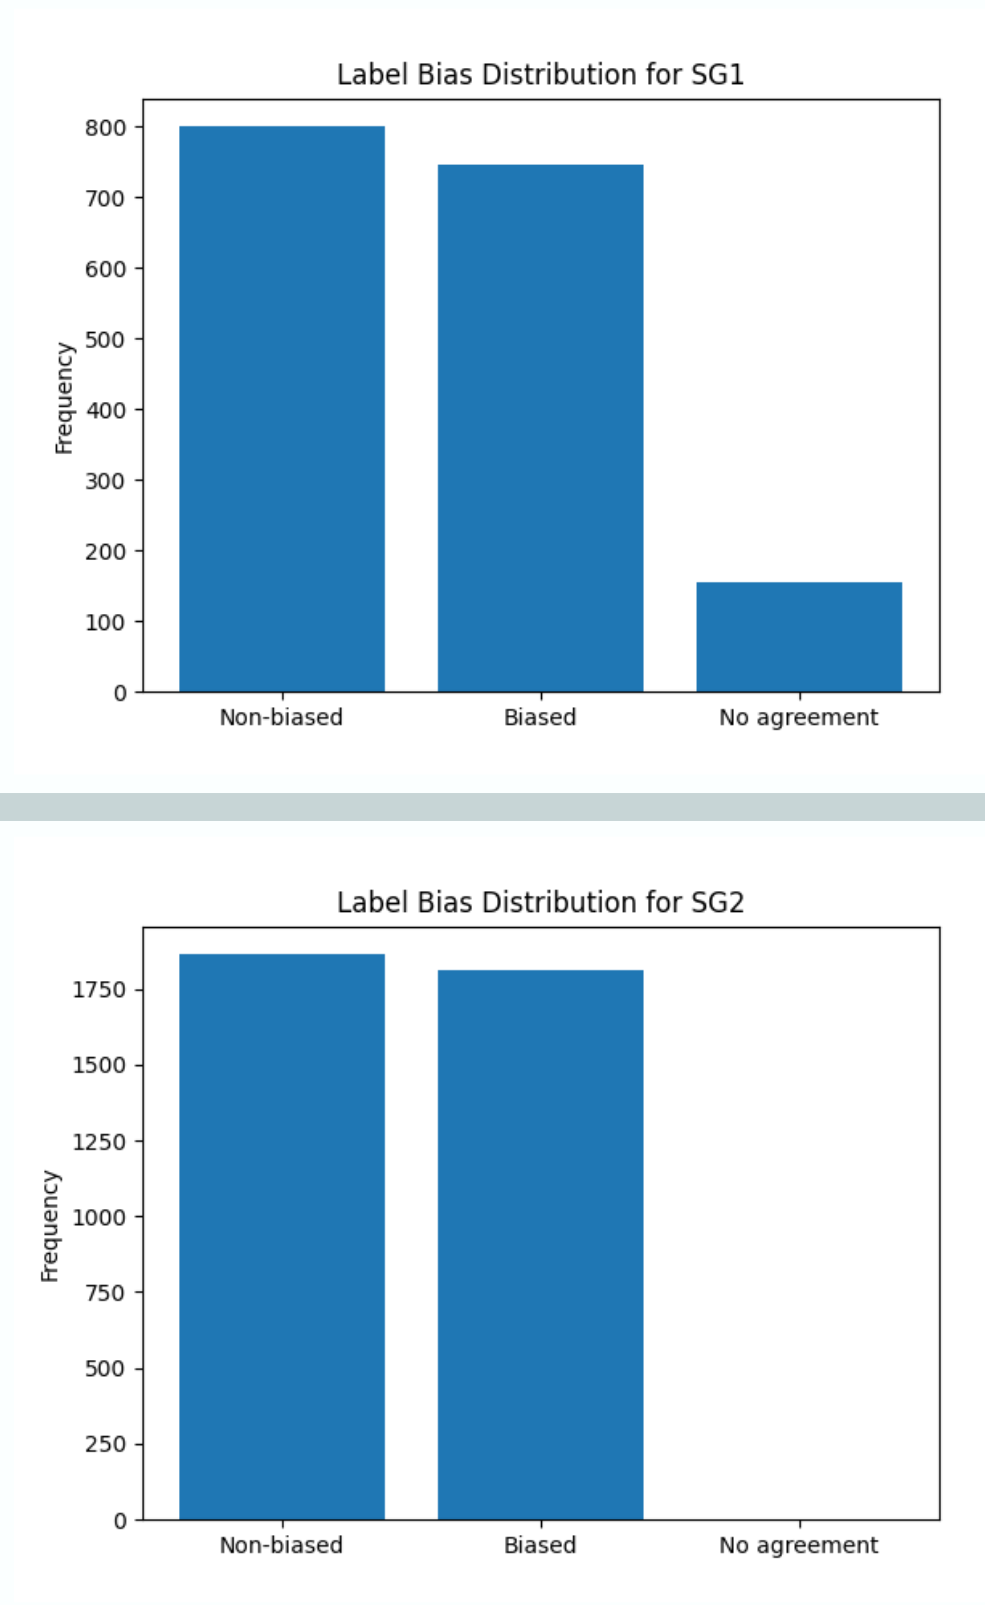
\includegraphics[width=0.5\textwidth]{SG_lb_bias.png}
\caption{Distribution of Bias across datasets}
\label{fig:my_label}
\end{figure}
Both datasets appear to have a similar amount of labels belonging to both classes.
The code for drawing the plots is available in the \text{'Datasetanalysis.ipynb'} in the repository.
Additionally, the count of label bias votes for each expert is given in Figure 2.
\begin{figure}[h]
\centering
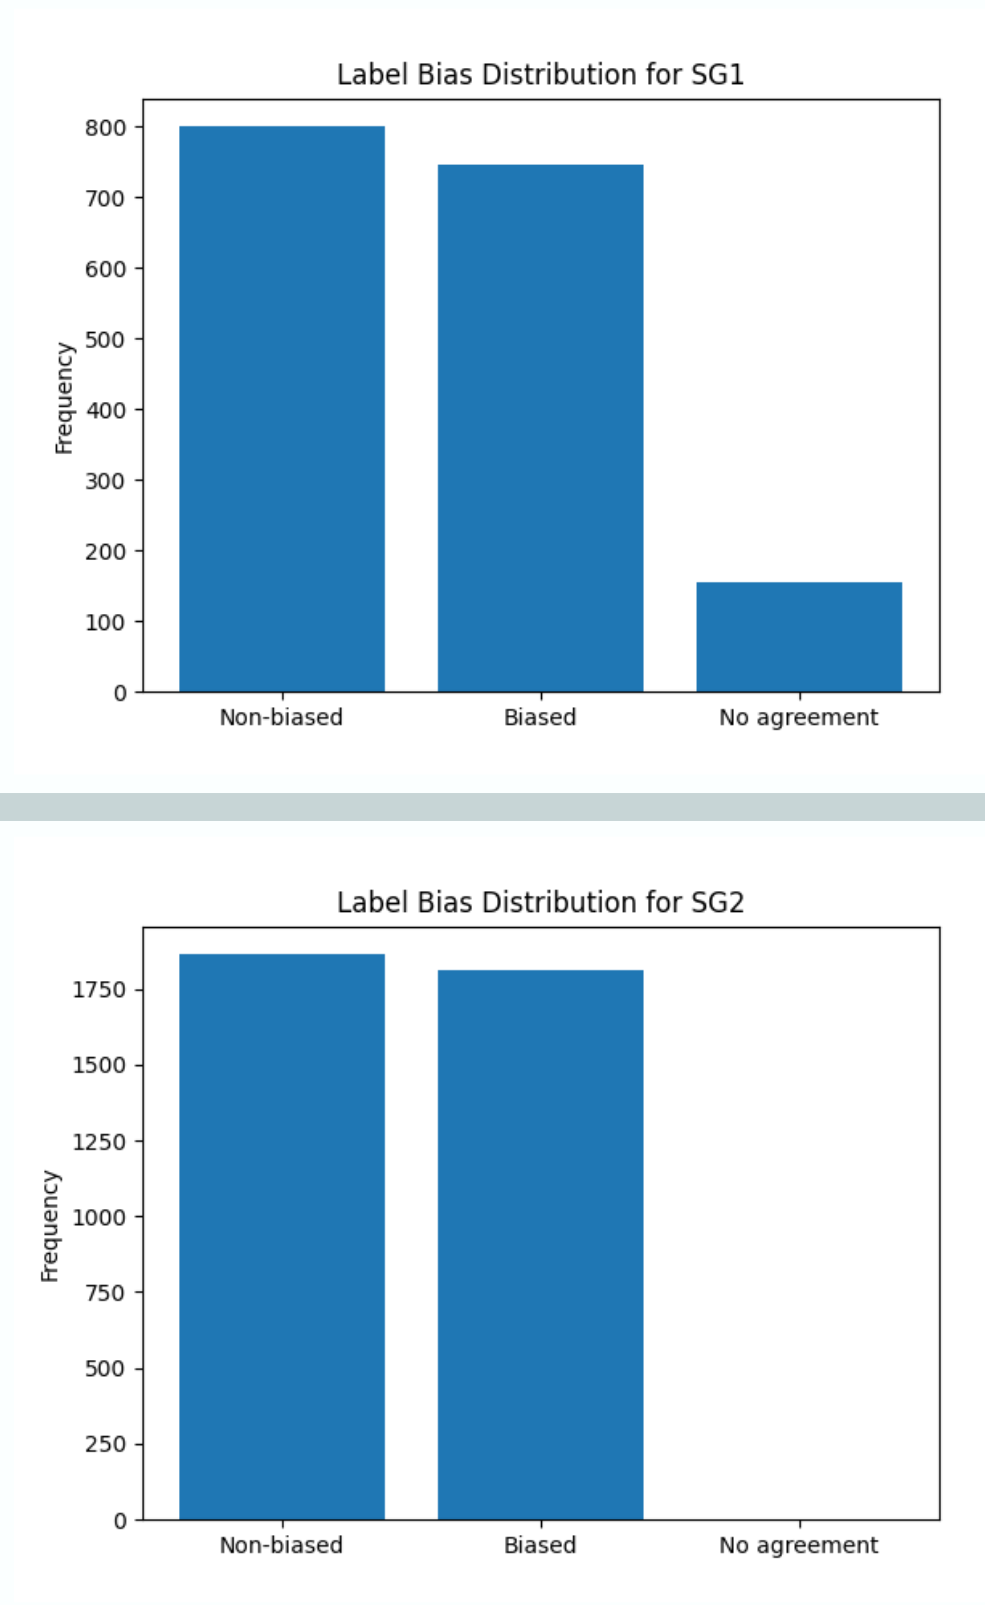
\includegraphics[width=0.5\textwidth]{SG_lb_bias.png}
\caption{Individuals label bias tagging for SG1 and SG2 subgroups}
\label{fig:my_label}
\end{figure}
In addition to these datasets, this project also contains scripts for extracting full-textual data from some news outlets. The data collection process for the evaluation phase of this project involved the extraction of textual data from news articles, specifically the title, highlight, and main body of each article. This was accomplished through the use of web scraping techniques, using the BeautifulSoup~\cite{richardson2007beautiful} to parse the HTML content of the web pages.

During the data collection process, certain challenges were encountered. Some of the links to the news articles were invalid or required the use of web proxies, rendering them inaccessible for the purposes of web scraping. To address this issue, these links were either replaced by querying the text of the article through the DuckDuckGo search engine, or they were discarded entirely.

Despite these challenges, the web scraping script performed effectively, extracting data from the majority of the available articles across various news outlets. The performance ensured enough data to analyze the model's behavior and also for the future needs of possible extensions of this study.\\
\\
\textbf{Notice}: The data extracted for this project is strictly used for academic purposes. It is used solely for the purpose of developing and evaluating machine learning models for media bias classification. No personal data is collected or used, and all data is handled in accordance with ethical guidelines and privacy standards.
\subsection{Models}
In this project, I employ a variety of models as a means of investigation for the main model. comprising three baseline models and a Large Language Model to perform text sequence classification. In the result section the models are compared according to the Accuracy, Precision, Recall, and F1 scores.
The Baseline models used here include:
\begin{itemize}
    \item \textbf{Majority Class classifier}: This is a simple classifier that always predicts the most frequent label in the training set. It does not learn any information from the input features and in literature it is often used as a baseline to compare with other (real) classifiers. It’s useful to provide a sanity check and to compare performance against the complex model.
    \item \textbf{Random Guesser}: This classifier generates predictions uniformly at random. The input features are not learned in this model as well. According to the dataset used in this project, using random predictions improves the results since the distribution of 'Biased' and 'Non-Biasd' are similar in this case. 
    \item \textbf{LogisticRegression}: Logistic Regression is a statistical model that uses logistic function to model binary variables. published the news article. This method calculates the probability of belonging to a class by learning from input. As a linear model, it is an effective solution to provide a baseline prediction of classes in the model.
\end{itemize}
The main methodology in this project follows the implementation as in ~\cite{spinde_2021_neural}. As the classifier RoBERTa~\cite{liu_2019_roberta} was implemented. RoBERTa is a variant of BERT which was trained on more data and for a longer amount of time. This model outperforms BERT and other state-of-the-art models on a variety of natural language processing tasks~\cite{a2020_overview}. The model was trained and evaluated on a Google Colab environment in several epochs through checkpointing. The specific hardware used in this project includes a V100 VRAM 16GB GPU and The default CPU, an Intel Xeon CPU with 2 vCPUs (virtual CPUs).
\subsection{Evaluation}
The evaluation of the model is a crucial aspect of this project, essentially providing a measure to show the goodness of the model's performance in bias identification tasks. The evaluation is divided into two subsections: 1- Traditional Evaluation Metrics and 2- Interpretive Model Evaluation.

\subsubsection{Traditional Evaluation Metrics}
In the first steps, the performance of models was tested using the most commonly used metrics. The metrics provide a comprehensive overview of performance while also considering both classes:
\begin{itemize}
    \item \textbf{Accuracy}: It is the ratio of correctly predicted observations to the total observations. It provides an intuitive measure of the overall correctness of the model:
    $$
    \text{Accuracy} = \frac{TP+TN}{TP+TN+FP+FN}
    $$
    \item \textbf{Precision}: This is the ratio of correctly predicted positive observations to the total predicted positive observations:
    $$
    \text{Precision} = \frac{TP}{TP+FP}
    $$
    \item \textbf{Recall}: Recall, or Sensitivity, is the ratio of correctly predicted positive observations to all observations in the actual class. It provides a measure of the model’s ability to find all the positive samples:
    $$
    \text{Recall} = \frac{TP}{TP+FN}
    $$
    \item \textbf{F1 Score}: It is the weighted average of Precision and Recall. It tries to find the balance between precision and recall and is particularly useful when dealing with imbalanced classes(The Classes in my dataset are mostly balanced):
    $$
    \text{F1} = \frac{2 \cdot \text{Precision} \cdot \text{Recall}}{\text{Precision} + \text{Recall}}
    $$
\end{itemize}
\subsubsection{Interpretative Model Evaluation}
In addition to the traditional metrics, a creative evaluation alternative is employed to provide a deeper understanding of the model’s performance. This alternative involves the use of the Anchors method for model interpretation.
Essentially, The Anchors method is a technique that can explain individual predictions of black-box classification by discovering a rule that sufficiently “anchors” the prediction locally – such that changes to the rest of the feature values of the instance do not matter~\cite{ribeiro_2018_anchors}.

\paragraph{Interpretation of Model Predictions on Extracted News Articles}
The second strategy involves extracting some news articles from the news articles in the original data, some using web scraping and some manually. The Anchors method is then run with the model’s predictions on these texts. 

This strategy allows for a more detailed analysis of the model’s decision-making process. By applying the Anchors method to individual sentences or sections within the articles, you can see which parts of the text the model is focusing on to make its predictions.
If the anchors identified in these new articles are similar to those found in the original dataset, it suggests that the model is applying what it has learned to new data. Conversely, if the anchors are very different, it could indicate that the model is struggling to generalize.
\section{Results}
This section presents the results of the fine-tuning process applied to the RoBERTa language model for the task of media bias classification.
\subsection{Model Fine-tuning}
The RoBERTa model was fine-tuned using a train-validation-test approach. This method ensures that each fold of the dataset contains an equal proportion of each targeted class, providing a robust estimate of the model’s performance.
\subsection{Handling Class Imbalance}
The two datasets used in this project did not exhibit class imbalance, however, after data splitting it was noted that some classes were under-represented in the data. This could lead to a model that performs well on the majority class but poorly on the minority class.

\begin{figure}[h]
    \centering
    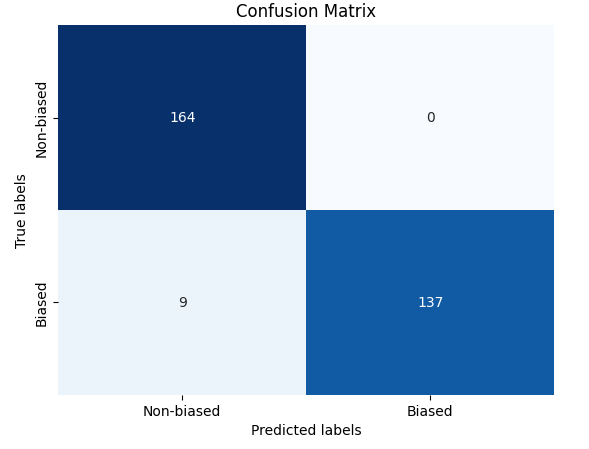
\includegraphics[width=0.9\linewidth]{cm_SG1_cl.png}
    \caption{confusion matrix for SG1 dataset with RoBERTa[value 1 indicate bias}
    \label{fig:enter-label}
\end{figure}

To address this issue, an oversampling method was implemented within each fold during the training process. Oversampling involves randomly duplicating examples from the minority class in the training data to balance the class distribution. This ensures that the model is exposed to enough examples of each class during training, improving its ability to generalize to under-represented classes.

After performing oversampling(please refer to Figure 3), the fine-tuned RoBERTa model was able to learn from a balanced representation of each class, leading to a more robust and reliable performance in the media bias classification task.
\subsection{Traditional Evaluation Metrics}
Considering the difference in the number of sentences within each dataset, they are analyzed separately, here is a brief summary of results from the SG1 dataset:
\begin{itemize}
    \item \textbf{Majority Class classifier}: It always predicts class 0. That’s why the recall for class 0 is 1.00 (it correctly identifies all instances of class 0), but the recall for class 1 is 0.00 (it fails to identify any instances of class 1). The overall accuracy of 0.54 indicates that 54\% of SG1 data belong to class 0.
    \item \textbf{Random Guesser}:  The precision, recall, and F1-score are roughly equal for both classes, indicating that it’s equally likely to guess either class. The overall accuracy of 0.53 is close to 0.5, as you’d expect from random guessing. 
    \item \textbf{LogisticRegression}: This model has a higher precision, recall, and F1-score for both classes compared to the other two classifiers, indicating that it is doing a better job of identifying both classes. The overall accuracy of 0.63 means it is correct about 63\% of the time.
\end{itemize}
In these numbers, macro avg was selected as the default averaging scheme for the metrics(the full result is present in {'finetuning.ipynb'}). Please note that the results of these algorithms do not necessarily indicate the distribution of labels in the corresponding dataset, this is mainly due to randomized train/test split before applying the models.

\begin{figure}
    \centering
    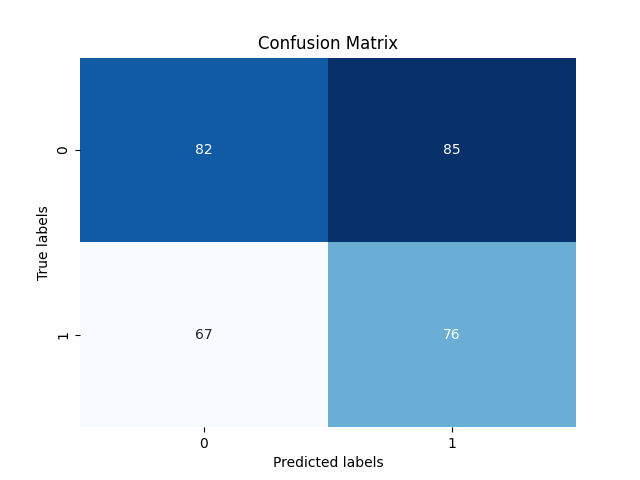
\includegraphics[width=0.9\linewidth]{cm_SG1_random_guess.png}
    \caption{confusion matrix belonging to the random guesses SG1[value 1 indicate bias]}
    \label{fig:enter-label}
\end{figure}
The metrics from the two datasets show a consistent pattern. Additionally, according to logistic regression results it can be observed that the increase in the number of data in each group has a substantial effect on learning from data.
On the other hand, the language model shows a very promising result for both SG1 and SG2 datasets. Regarding the SG1 dataset, the model exhibits an accuracy rate of 0.97 which is significantly better all the baselines, similarly, a recall of 0.94 suggests that the model identifies only 94\% of all True positive instances.
In this context we need to improve the rate of correctly predicted bias labels, therefore we have to maximize accuracy and precision to enhance the overall correctness and lower the false positive rate.

\begin{table*}[h]
\caption{Baselines macro avg results across datasets}
\small
\centering
\begin{tabular}{llllll}
{\color[HTML]{000000} Model name} & {\color[HTML]{000000} Accuracy} & {\color[HTML]{000000} Precision} & {\color[HTML]{000000} Recall} & F1   & Dataset \\
Majority Class                                           & 0.54                                                   & 0.27                                                    & 0.50                                                 & 0.35 & SG1     \\
Random Guesser                                           & 0.53                                                   & 0.53                                                    & 0.53                                                 & 0.53 & SG1     \\
Logistic Regression                                      & 0.63                                                   & 0.63                                                    & 0.63                                                 & 0.63 & SG1     \\
Majority Class                                           & 0.51                                                   & 0.26                                                    & 0.50                                                 & 0.34 & SG2     \\
Random Guesser                                           & 0.53                                                   & 0.53                                                    & 0.53                                                 & 0.53 & SG2     \\
Logistic Regression                                      & 0.71                                                   & 0.71                                                    & 0.71                                                 & 0.71 & SG2    
\end{tabular}
\end{table*}

\begin{table*}[h]
\caption{language model performance metrics}
\centering
\begin{tabular}{ccccccc}
Loss & \multicolumn{1}{l}{Accuracy} & \multicolumn{1}{l}{Precision} & \multicolumn{1}{l}{Recall} & \multicolumn{1}{l}{Micro F1} & \multicolumn{1}{l}{Weighted F1} & \multicolumn{1}{l}{Dataset} \\
0.08 & 0.97                         & 1                             & 0.94                       & 0.97                         & 0.97                            & SG1                         \\
0.19 & 0.94                         & 0.95                          & 0.92                       & 0.94                         & 0.94                            & SG2                        
\end{tabular}
\end{table*}
\subsection{Interpretative Model Evaluation}
In this section, the model is evaluated using a variety of text among the extracted data from news articles. Here are six chosen examples from the SG2 dataset that demonstrate the model capabilities:
\begin{itemize}
    \item 'Civil rights activists across the United States for years have called for scaling back traditional policing, and the efforts have gained momentum...': This is an instance of Non-biased text, the model classifies it as Non-Biased, Anchors method chose 'protests', 'called', and 'gained' as the indicator for this decision
    \item 'An attorney for President Donald Trump on Friday blasted U.S. House Democrats’ request for six years of Trump’s tax returns as “a misguided attempt” to politicize...': This is an instance of Biased text. The experts identified the keyword 'blasted' as the indicator for bias, RoBERTa classified this sentence as Biased, and based on Anchors the decision is also based on the 'blasted' keyword.
    \item 'Japan has reported about 1300 deaths from COVID-19 but new cases in Tokyo have fallen in the last few weeks': This instance was extracted from a news article. Based on the model prediction this is Non-Biased and the indicator is the keyword 'reported'. This is likely true since it is a factual text and presents information about the trend of new cases in Japan.
    \item 'The idea of a "rigged" economy that both benefits and is shaped by the rich and powerful was a popular theme in 2016 and is sure to play a big role again this cycle...': This is a second instance extracted from news articles. The model predicted Non-Biased with Anchors indicators of {powerful, popular, emphasizing, big, several, idea, shaped, candidates, campaign, economy, rich, sure, rigged, ...}. After looking at the corresponding text, it is most likely a False Negative. This sentence offers a subjective viewpoint and uses the words 'Rigged', 'Rich', and 'powerful' to imply a negative view of the corresponding groups.
    \item 'As you know, this is a very high priority for the president, ending surprise medical bills': The model predicts this instance as Non-Biased and the anchor indicators are {very, surprise, medical, ...}. This is factual information, so it is True Positive.
    \item 'The findings suggest childhood vaccination efforts nearly ground to a halt between March 13 — when the national emergency was declared — and April 19': The model predicted this text as Non-biased with the Anchors keyword of 'childhood'. This proved to be a True sentence after a web search.
\end{itemize}
\section{Conclusion and Discussion}
This project aimed to classify media bias in news articles using a fine-tuned RoBERTa model and compare its performance with three baseline models. The results demonstrated the effectiveness of the RoBERTa model in this task greatly. As expected, the model performed better on the SG1 dataset due to a smaller overall amount of annotated sentences.

In addition to traditional evaluation metrics, an interpretative evaluation strategy was employed to provide a deeper understanding of the model’s decision-making process. The Anchors method was used to identify the words that the model relied on most heavily to make its predictions, providing insight into what the model had learned and how it was making its decisions.

Regarding the limitations of this work, firstly, despite the effectiveness of RoBERTa model in bias identification, the model the training process was computationally expensive due to the complexity of the model, potentially limiting its accessibility.\\
Secondly, for the sampling step of anchor $en_core_web_md$ model from spaCy was used. Larger models(such as $en_core_web_lg$) have more parameters and potentially richer word vectors, which might lead to different perturbations being generated during the sampling process, this could be a potential direction for future improvements.\\
Lastly, the original labels annotated by experts was categorized to 'Biased', 'Non-Biased', and 'No agreement'. The third class indicates uncertainty or lack of consensus among experts, which could introduce additional noise; Therefore to improve consistency the labels from the third class were removed before the finetuning process. This is not problematic due to the very small population of this class, a more sophisticated approach would be to employ consensus-building techniques among experts to resolve disagreements before labeling.\\
Additionally, another research direction for this project would be to look more into the interpretation of the model's behavior including the use of other model-agnostic methods.

Overall, this project demonstrates the potential of transformer-based models like RoBERTa in the task of media bias classification. It also highlights the importance of interpretability in machine learning, showing how methods like Anchors can prove valuable. The provided mode can help readers and journalists understand and check for biases, contributing to more informed public discourse.
\newpage
\bibliography{anthology,acl2020}
\bibliographystyle{acl_natbib}
\end{document}
